On Problem Set~10, you solved the heat equation on a two-dimensional square domain.
Now we will investigate the wave equation on the same domain,
a model of a vibrating membrane stretched over a square frame---that 
is, a square drum:
\[ u_{tt}(x,y,t) = u_{xx}(x,y,t) + u_{yy}(x,y,t),\]
with $0\le x\le 1$, and $0\le y\le 1$, and $t\ge 0$.
Take homogeneous Dirichlet boundary conditions
\[ u(x,0,t) = u(x,1,t) = u(0,y,t) = u(1,y,t) = 0\]
for all $x$ and $y$ such that $0\le x\le 1$ and $0\le y\le 1$ and all $t\ge 0$,
and consider the initial conditions
\[  u(x,y,0) = u_0(x,y) = \sum_{j=1}^\infty \sum_{k=1}^\infty a_{j,k}(0) \psi_{j,k}(x,y), 
       \qquad
   u_t(x,y,0) = v_0(x,y) 
               = \sum_{j=1}^\infty \sum_{k=1}^\infty b_{j,k}(0) \psi_{j,k}(x,y).\]
      Here $\psi_{j,k}(x,y) = 2 \sin(j \pi x)\sin(k \pi y)$, 
      for $j, k\ge 1$,  are the eigenfunctions of the operator
       \[ L u = -(u_{xx} + u_{yy}),\]
      with homogeneous Dirichlet boundary conditions, as in Problem Set~10.
      You may use without proof that these eigenfunctions are orthogonal, 
      and use the eigenvalues $\lambda_{j,k} = (j^2+k^2)\pi^2$ computed 
      for Problem Set~10.

\begin{enumerate}
\item We wish to write the solution to the wave equation in the form
       \[ u(x,y,t) = \sum_{j=1}^\infty \sum_{k=1}^\infty a_{j,k}(t) \psi_{j,k}(x,y).\]
      Show that the coefficients $a_{j,k}(t)$ obey the ordinary differential equation
       \[ a_{j,k}''(t) = -\lambda_{j,k} a_{j,k}(t) \]
      with initial conditions
       \[ a_{j,k}(0), \qquad
         a'_{j,k}(0) = b_{j,k}(0)\]
      derived from the initial conditions $u_0$ and $v_0$.

\item Write down the solution to the differential equation in part~(a).

\item Use your solution to part~(b) to write out a formula for the solution $u(x,y,t)$.
       
\item Suppose the drum begins with zero velocity, $v_0(x,y)=0$, and displacement
         \[ u_0(x,y) = 200xy (1-x) (1-y)(x-1/4)(y-1/4) 
                     = \sum_{j=1}^\infty \sum_{k=1}^\infty 
                        {100 (5+7(-1)^j)(5+7(-1)^k)\over j^3 k^3 \pi^6} \psi_{j,k}(x,y). \]

      Submit surface (or contour) plots of the solution at times 
      $t=0, 0.5, 1.0, 1.5, 2.5$, using $j=1,\ldots,10$ and $k=1,\ldots,10$
      in the series.
\end{enumerate}
%%%%%%%%%%%%%%%%%%%%%%%%%%%%%%%%%%%%%%%%%%%%%%%%%%%%%%%%%%%%%%%%%%%%%%%%%%%%%%%%

\ifthenelse{\boolean{showsols}}{\begin{solution}
This question follows the same pattern as the first problem on this problem set.
\begin{enumerate}
\item Substitute the formula
       \[ u(x,y,t) = \sum_{j=1}^\infty \sum_{k=1}^\infty a_{j,k}(t) \psi_{j,k}(x,y).\]
      into the two dimensional wave equation to obtain
        \[ \sum_{j=1}^\infty \sum_{k=1}^\infty 
              {d^2 a_{j,k}\over d t^2} (t) \psi_{j,k}(x,y) 
          = \sum_{j=1}^\infty \sum_{k=1}^\infty 
               a_{j,k}(t) \Big({\d^2 \over \d x^2} + {\d^2 \over \d y^2}\Big)\psi_{j,k}(x,y),\]
       which implies
        \[ \sum_{j=1}^\infty \sum_{k=1}^\infty 
              {d^2 a_{j,k}\over d t^2} (t) \psi_{j,k}(x,y) 
          = \sum_{j=1}^\infty \sum_{k=1}^\infty 
               -a_{j,k}(t) \lambda_{j,k} \psi_{j,k}(x,y).\]
        Take the inner product of both sides with $\psi_{m,n}$ and use the orthogonality
        of the eigenfunctions to obtain
         \[ a''_{j,k}(t)  = -\lambda_{j,k} a_{j,k}(t).\]
        The initial value $a_{j,k}(0)$ is simply the $(j,k)$ coefficient in the
         expansion of the initial condition,
\[  u(x,y,0) = u_0(x,y) = \sum_{j=1}^\infty \sum_{k=1}^\infty a_{j,k}(0) \psi_{j,k}(x,y). \]
        As the differential equation describing $a_{j,k}$ is of second order, 
        we require a second initial condition to determine a unique solution.
        Since 
          \[ u_t(x,y,0) = \sum_{j=1}^\infty \sum_{k=1}^\infty a'_{j,k}(0) \psi_{j,k}(x,y),\] 
        and 
          \[ v_0(x,y) = \sum_{j=1}^\infty \sum_{k=1}^\infty b_{j,k} \psi_{j,k}(x,y),\]
        the second initial condition we require is simply the $(j,k)$ coefficient of $v_0$:
          \[ a'_{j,k}(0) = b_{j,k}.\]
         
\item As we have seen often in this class, the equation $a''_{j,k}(t) = -\lambda_{j,k} a_{j,k}(t)$
      has solutions of the form
       \[ a_{j,k}(t) = A \sin(\sqrt{\lambda_{j,k}} t) + B \cos(\sqrt{\lambda_{j,k}} t),\]
      with $A$ and $B$ determined by the initial conditions.
      In particular, evaluating the general solution at $t=0$ immediately gives
       \[B = a_{j,k}(0).\]
      Computing the derivative
       \[ a'_{j,k}(t) = A \sqrt{\lambda_{j,k}} \cos(\sqrt{\lambda_{j,k}} t) 
                        - B \sqrt{\lambda_{j,k}} \sin(\sqrt{\lambda_{j,k}} t)\]
       and evaluating it at $t=0$ then gives
       \[ A = {b_{j,k}(0)\over \sqrt{\lambda_{j,k}}}.\]


\item From this formula for $a_{j,k}(t)$ we obtain the solution
\[ u(x,t) = \sum_{j=1}^\infty \sum_{k=1}^\infty
                 \Big[\Big({b_{j,k}(0) \over \sqrt{\lambda_{j,k}}}\Big)
                   \sin(\sqrt{\lambda_{j,k}} t) + a_{j,k}(0) \cos(\sqrt{\lambda_{j,k}} t)\Big]
                    \big(2 \sin(\sqrt{\lambda_{j,k}} x)\sin(\sqrt{\lambda_{j,k}} y)\big).\]

\item Zero initial velocity implies that $b_{j,k}(0) = 0$ for all $(j,k)$ pairs.
      The solution thus simplifies to
\[ u(x,t) = \sum_{j=1}^\infty \sum_{k=1}^\infty
                   a_{j,k}(0) \cos(\sqrt{\lambda_{j,k}} t)
                    \big(2 \sin(\sqrt{\lambda_{j,k}} x)\sin(\sqrt{\lambda_{j,k}} y)\big).\]
      with 
      \[ a_{j,k}(0) = {100 (5+7(-1)^j)(5+7(-1)^k)\over j^3 k^3 \pi^6}.\]

\begin{center}
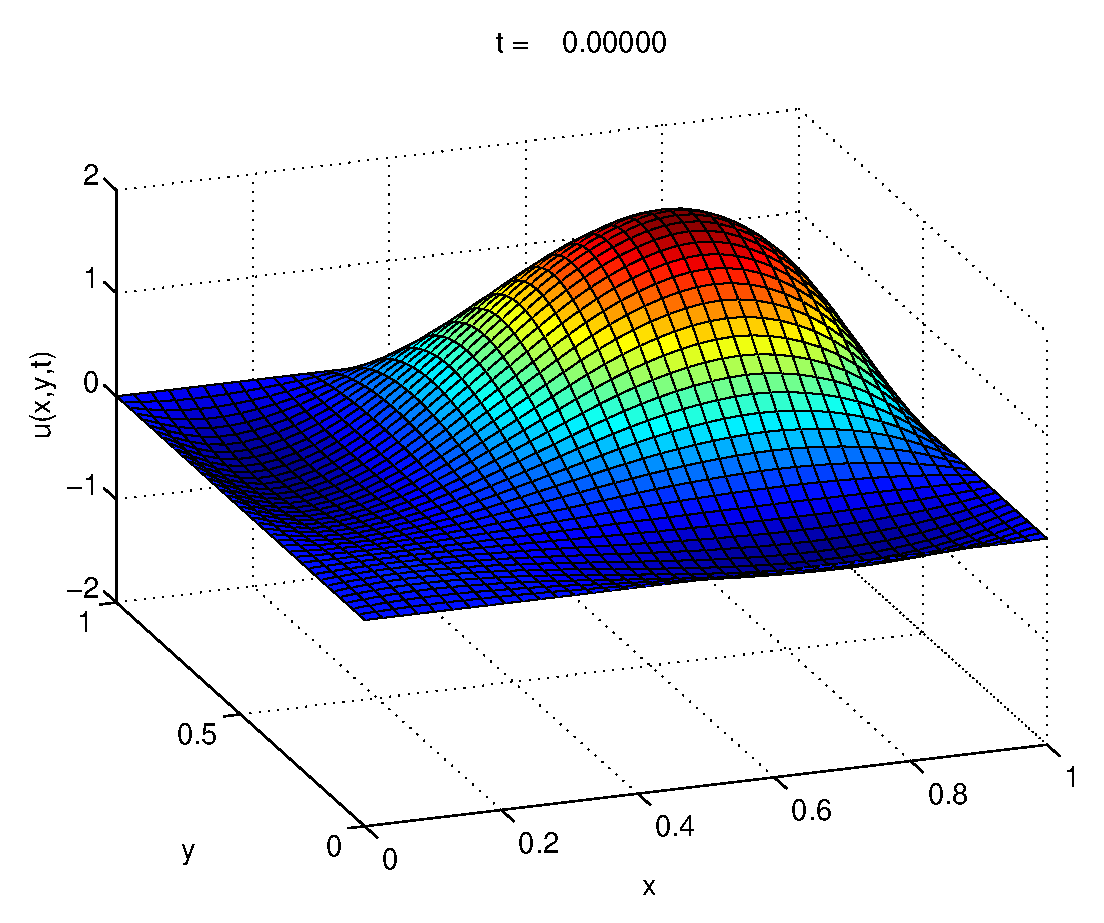
\includegraphics[scale=0.37]{wave2d_1} \quad
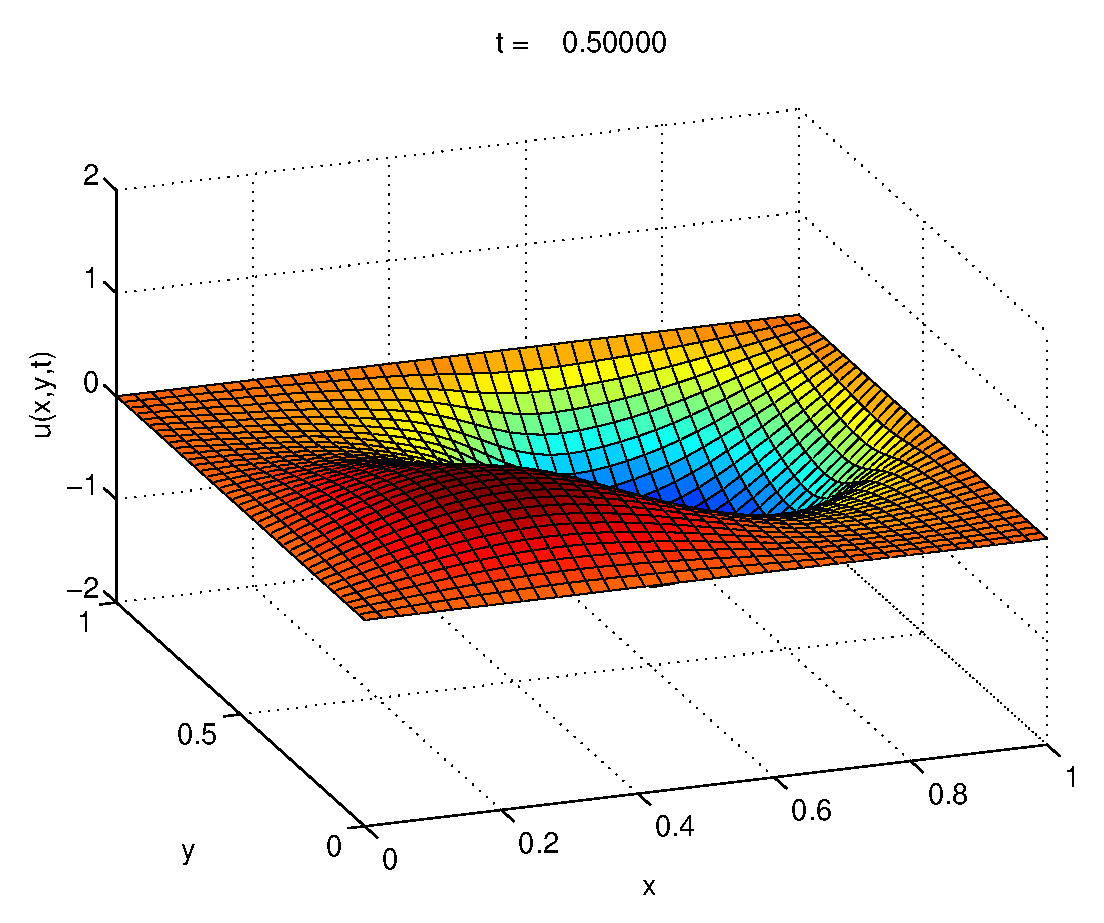
\includegraphics[scale=0.37]{wave2d_2} 

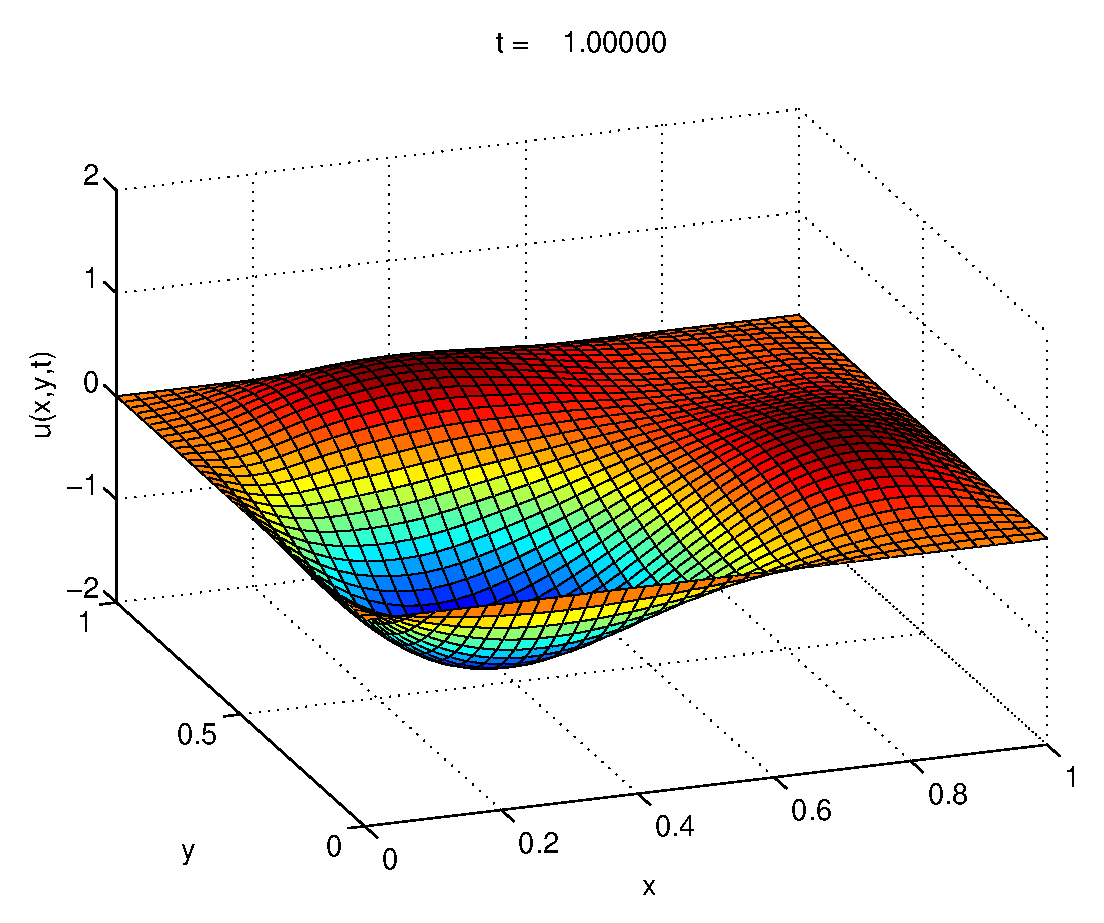
\includegraphics[scale=0.37]{wave2d_3} \quad
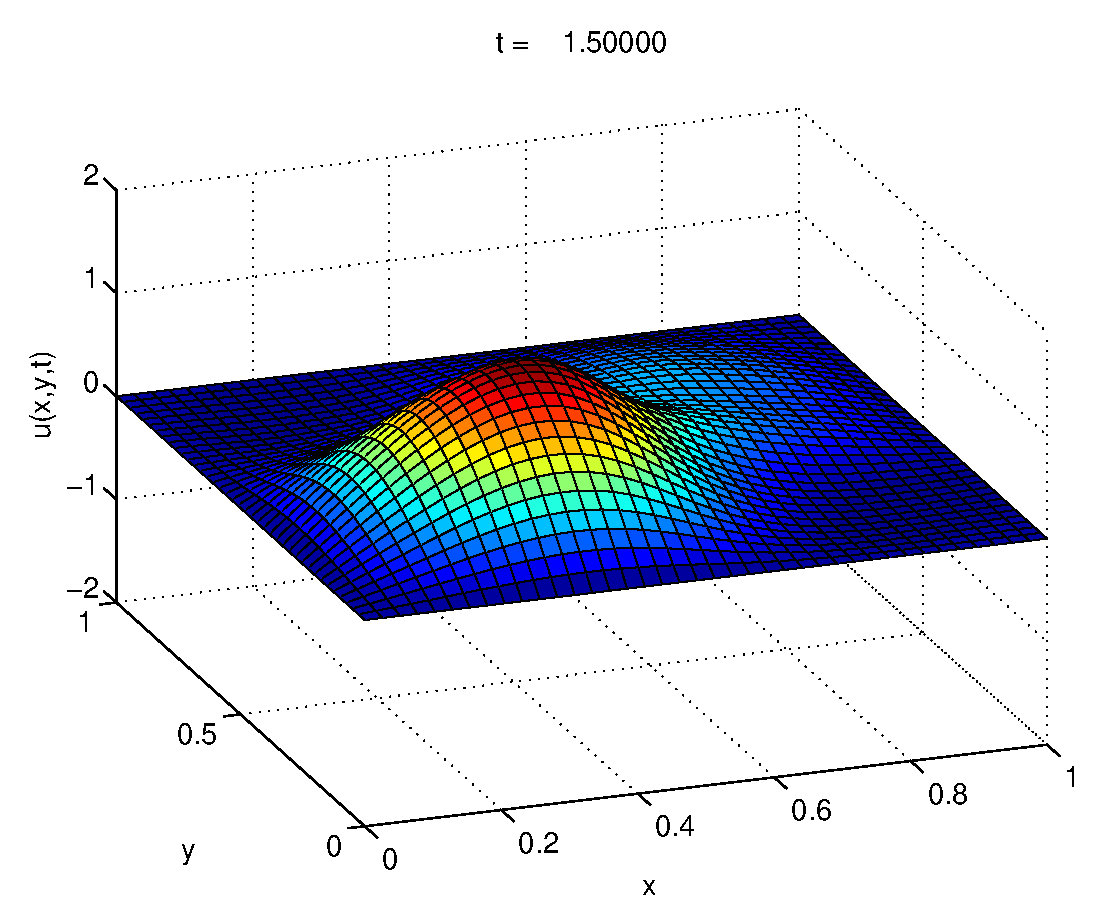
\includegraphics[scale=0.37]{wave2d_4} 

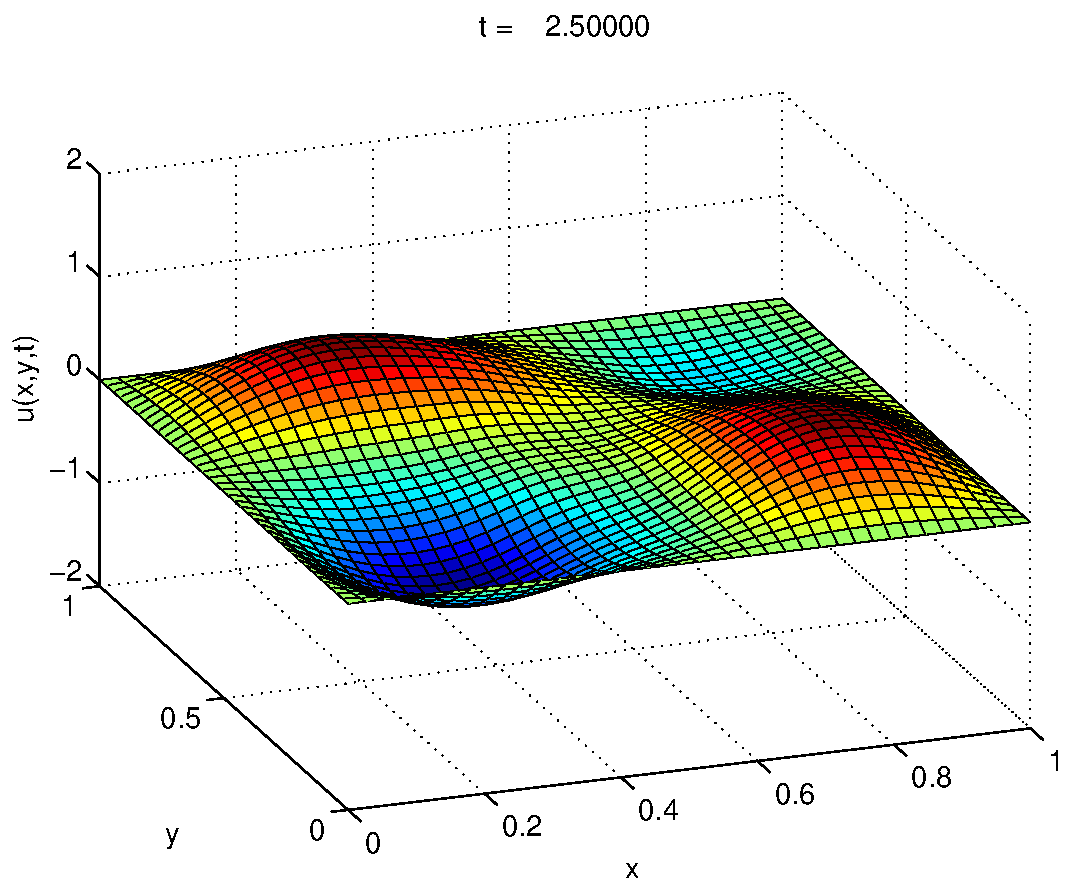
\includegraphics[scale=0.37]{wave2d_5} 
\end{center}

\newpage
The code that produced these plots follows.

\input wave2d_code
\end{enumerate}
\end{solution}}{}

